
 Beyond the physics of single hadrons described in the previous sections, the wealth of complexity embodied in the nuclear landscape emerges from QCD and the other forces of the SM.  From the point of view of QCD, this emergence is an interesting phenomena, with the various effective degrees of freedom in nuclei (nucleons, $\alpha$ clustering, shells, resonances) all being extremely non-trivial consequences of QCD dynamics that beg for explanation. The first steps in addressing this complexity from LQCD have been made over the last decade, and we anticipate that LQCD will be an increasingly important part of nuclear theory in the coming years. Since the SM forms the foundation of nuclear physics, LQCD can be used to study the forces that bind nucleons into nuclei and govern their interaction, as well as to investigate how nuclear systems interact with external electroweak probes and possible physics beyond the Standard Model.
While there has been remarkable progress in this area over the last decade, it is clearly an area where major opportunities for new developments exist and major challenges await.

\subsection{Nuclear spectroscopy}

Determining the ground state energies and bindings of light nuclei is a central challenge for LQCD in nuclear physics. The very first LQCD calculations of nuclei (objects with baryon number greater than one) are less than a decade old and significant advances in the study of nuclear systems have occurred over the last five years. Although no bound states were determined, earlier studies of baryon-baryon systems \cite{Yamazaki:2009ua,Beane:2006gf,Beane:2006mx,Beane:2009gs,Beane:2009kya}  developed the necessary contraction and analysis techniques for efficient study of two-body systems. 
The first calculations of bound systems with baryon number $A\ge2$ were of the doubly-strange $H$-dibaryon system at unphysical quark masses \cite{Beane:2010hg,Inoue:2010es,Beane:2011xf}. 
Studies of the two-nucleon channels \cite{Beane:2011iw} and other exotic channels were performed subsequently \cite{Berkowitz:2015eaa,Francis:2018qch,Wagman:2017tmp}. These studies used the same L\"uscher method discussed above in Section \ref{sec:hadronspectroscopy}, converting finite volume energy eigenvalues into determinations of infinite volume bound state pole positions. Bound states have also been found using HAL potential method \cite{Ishii:2006ec} based on Refs.~\cite{Luscher:1986pf,Lin:2001ek}, although issues with the validity of current applications of the method have been raised  \cite{Detmold:2007wk,Birse:2012ph,Yamazaki:2018qut,Yamazaki:2017gjl,Namekawa:2017sxs} and it is only recently that systematics have begun to be addressed in this method \cite{Kawai:2017goq}.
A series of studies of systems of many mesons \cite{Beane:2007es,Detmold:2008yn,Detmold:2011kw} extracted a three-particle interaction from LQCD for the first time.
Calculations of systems up to atomic number $A=4$  have ensued \cite{Beane:2012vq,Yamazaki:2012hi,Yamazaki:2015asa}, with almost physical quark mass calculations being currently performed by the PACS-CS collaboration \cite{Yamazaki:2015asa}. The authors of Refs.~\cite{Iritani:2018zbt} have suggested that systematic issues exist in the extractions of energies in many of these studies. While such issues can potentially exist they require careful investigation on a case-by-case basis and many aspects of the criticism are refuted for particular calculations in Refs.~\cite{Beane:2017edf,Namekawa:2017sxs,Yamazaki:2017jfh}.

Spectroscopy of nuclear systems is particularly challenging for LQCD for multiple reasons, some physical and others technical. The first challenge stems from the fact that the physics of nuclei is complicated, with low-energy excitations possible through many different mechanisms; understanding even the simplest aspects completely requires precision control. Existing studies are at some level saved by the finite volumes and the heavier than physical quark masses that were used which lead to a simpler spectrum. However future calculations in large volumes and with physical quark masses must confront these issues (Ref.~\cite{Beane:2012vq} highlights just how formidable this challenge is).
A second challenge arises from the Monte-Carlo nature of LQCD calculations. As emphasised by Parisi and Lepage \cite{Lepage:1989hd,Parisi:1983ae,Hamber:1983vu}, single baryon correlation functions exhibit a signal-to-noise ratio that degrades exponentially with the temporal separation. For nuclear systems, the problem only becomes more challenging \cite{Beane:2009kya,Beane:2009gs} and extraction of the eigenenergies is consequently difficult. A number of methods have been developed that aim to ameliorate this issue, either defining better-behaved estimators \cite{Beane:2014oea,Wagman:2017gqi,Wagman:2017xfh,Wagman:2016bam,Detmold:2018eqd} or new analysis strategies that optimize the ratio of signal to noise \cite{Detmold:2014hla}. None of these methods has completely solved the signal-to-noise problem, but have proved sufficient for studies of the lightest few nuclei. 
Finally, at least naively, the complexity of contractions grows 
factorially with the system size; calculations for $^4$He are at first sight $6!6!/2\sim 260,000$ times  more difficult than for a proton. Efforts to reduce these costs have enabled the progress described above and have proceeded via construction of enumerative \cite{Doi:2012xd,Gunther:2013xj} and recursive \cite{Detmold:2010au,Detmold:2012eu} algorithms. 
Given the exponentially hard nature of these challenges, new techniques making use of machine learning and also quantum information science will potentially have transformative  impact 
in  many body lattice QCD in particular. Some new directions are discussed in the companion White Paper on Computational Lattice Field Theory.


There are many opportunities for increased effort in this area as well as many technical challenges that exist in going to larger systems and performing calculations at the physical quark masses. 
Extending existing calculations to even moderately larger $A$ will have significant impact as nuclei that require $p$-shell configurations become accessible. These systems depend on more complicated aspects of the nuclear forces than the $A\le4$ nuclei that have been studied and new lattice calculations will be useful in constraining different spin and isospin components of these forces. Larger nuclei also exhibit interesting collective effects such as halo structures (eg,  ${}^{6,8}$He), cluster structures (eg ${}^{8}$Be, ${}^{12}$C) and deformations that would be very instructive to see emerge from LQCD calculations.  Extension of the current calculations to excited states of nuclear systems will also provide renewed insight into the nature of nuclei but will require exascale computing and advanced variational techniques such as those discussed in Section \ref{sec:hadronspectroscopy}.
By using a large basis of operators of different symmetries and structures, this would allow a detailed understanding the nature of these excitations and the origin of collectivity in nuclei. 

LQCD offers the possibility of investigating nuclei away from the physical quark masses, or for different gauge and fermion content of the theory, as an intellectual pursuit of its own. These systems cannot be studied in experiment, but can provide a broader perspective on the nature of gauge filed theories and concrete answers to questions related to the naturalness of nuclear physics \cite{Orginos:2015aya,Epelbaum:2012iu,Berengut:2013nh,CarrilloSerrano:2012ja}. With the  possibility of strongly interacting gauge theories other than QCD occurring in the context of dark matter and hidden valley models, it is also interesting to understand how ubiquitous nuclear physics is and whether there are QCD-like theories that do not exhibit nuclear physics.  In a first step in this direction,  Refs.~\cite{Detmold:2014qqa,Detmold:2014kba}  consider $N_f=N_c=2$ QCD and examine the nuclear physics and phenomenological consequences of  a putative dark matter sector based on this theory. Surprisingly these studies, and studies of $N_c=3$ QCD at unphysical quark masses suggest that the shallow binding of nuclei is a fairly generic phenomenon in theory space. Further investigations of theories such as those with multiple matter representations \cite{Niel} may display fundamentally different nuclear phenomena.



\subsection{Nuclear Structure}
\label{sec:nuclearstructure}

Exploration of the structure of the nuclei found in LQCD calculations from the underlying quark and gluon degrees of freedom offers  opportunities for new insight as well as additional challenges.  Phenomenologically, the spectroscopy and decay patterns of excitations of nuclei have been an important source of structure information. However, interactions of nuclei with electroweak probes have provided the most precise information we have about nuclear structure. 
In particular, the magnetic moments,  higher multiple moments and polarizabilities  have enabled a static picture of nuclei to be determined. The electromagnetic form factors of nuclei have revealed their charge and current distributions and  have further
developed our understanding of nuclear structure. 
Nuclear parton distributions extracted from deep-inelastic scattering on nuclear targets provides a different perspective on the partonic substructure of nuclei. Based on this phenomenology, nucleons are seen to be effective degrees of freedom inside nuclei, leading to the success of many-body approaches based on nucleon degrees of freedom in describing many aspects of nuclear structrue. However, there are many ways in which nuclei reveal that non-nucleonic degrees of freedom are important inside the nucleus. The EMC effect \cite{Aubert:1983xm}, discovered in 1983, is perhaps the most striking; it shows that the distribution of quarks and gluons in a nucleus differs at the ${\cal O}(20\%)$ level from the incoherent sum of the distributions in the nucleon. Understanding these and other aspects of nuclear structure from QCD  BLAHBLAH

%
\begin{figure}[!t]
	\centering
	\raisebox{0.1\height}{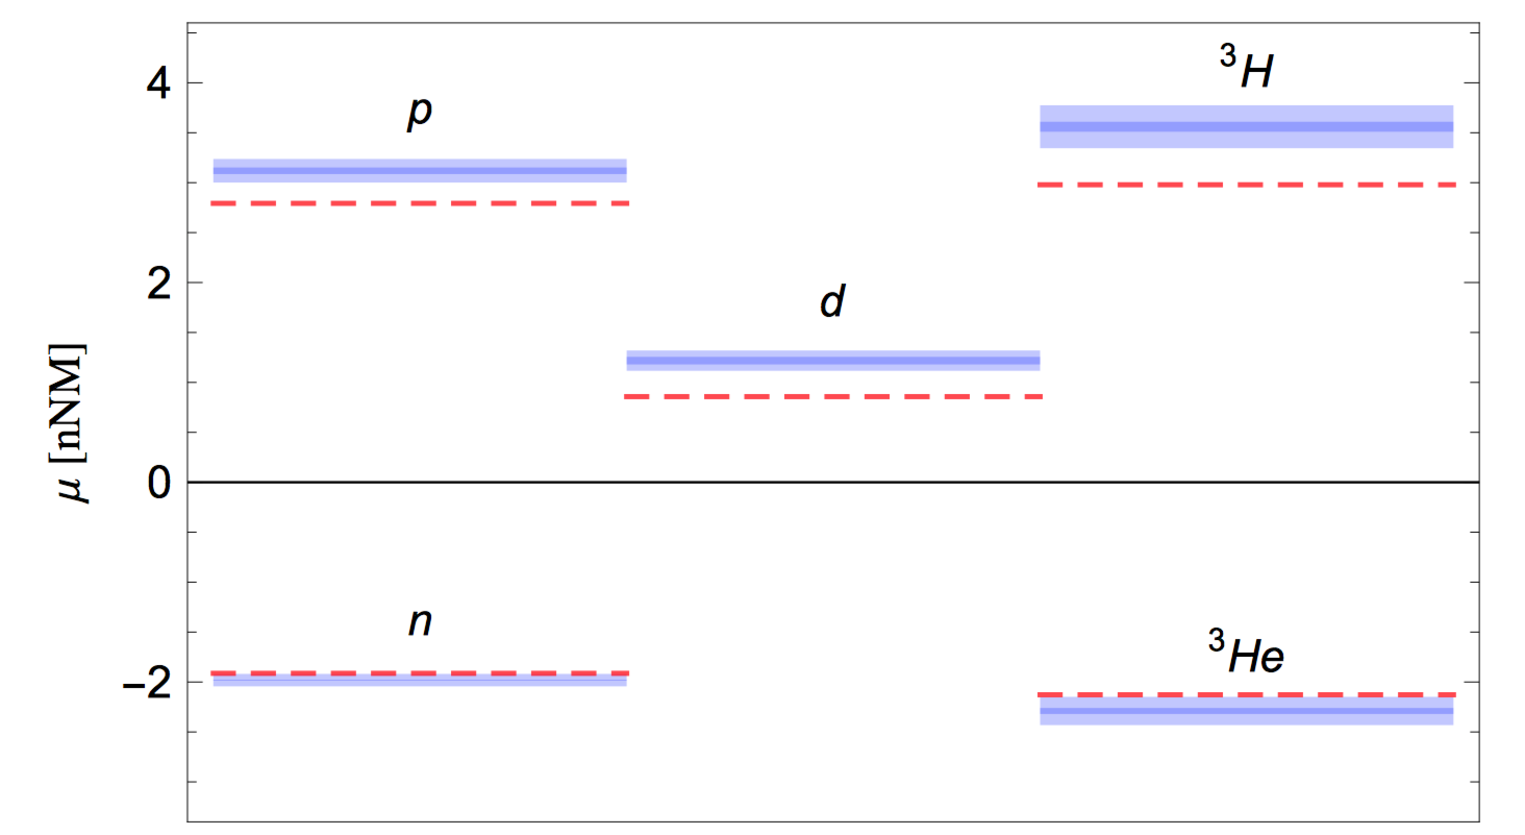
\includegraphics[width=0.48\columnwidth]{figures/MagMoms.pdf}  }
	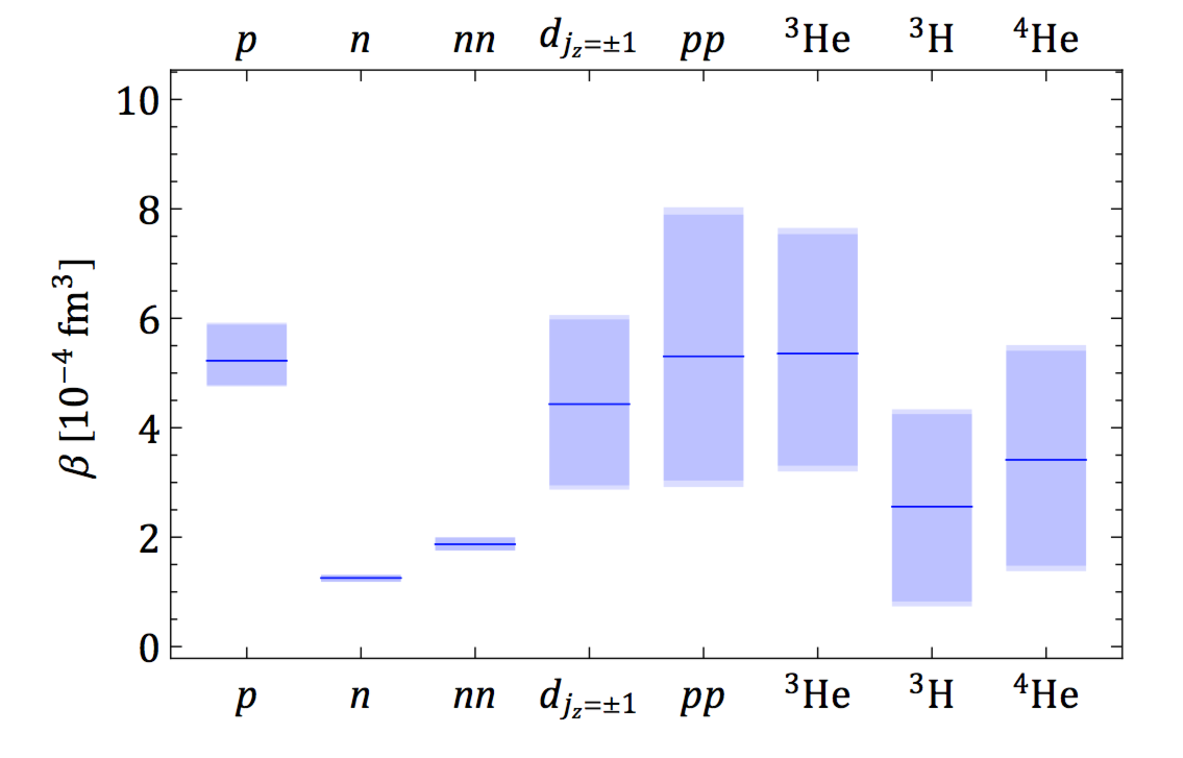
\includegraphics[width=0.49\columnwidth]{figures/PhysPols.pdf}
	\caption{ 
		A summary of the magnetic moments~\protect\cite{Beane:2014ora} (left panel) and polarizabilities (right panel) of the nucleons and
		light nuclei calculated with LQCD at a pion mass of
		$m_\pi\sim 805~{\rm MeV}$~\protect\cite{Chang:2015qxa}.    }
	\label{fig:summaryBETA}
\end{figure}

%
\begin{figure}{r}
	\vspace*{-0cm}
	\centering
	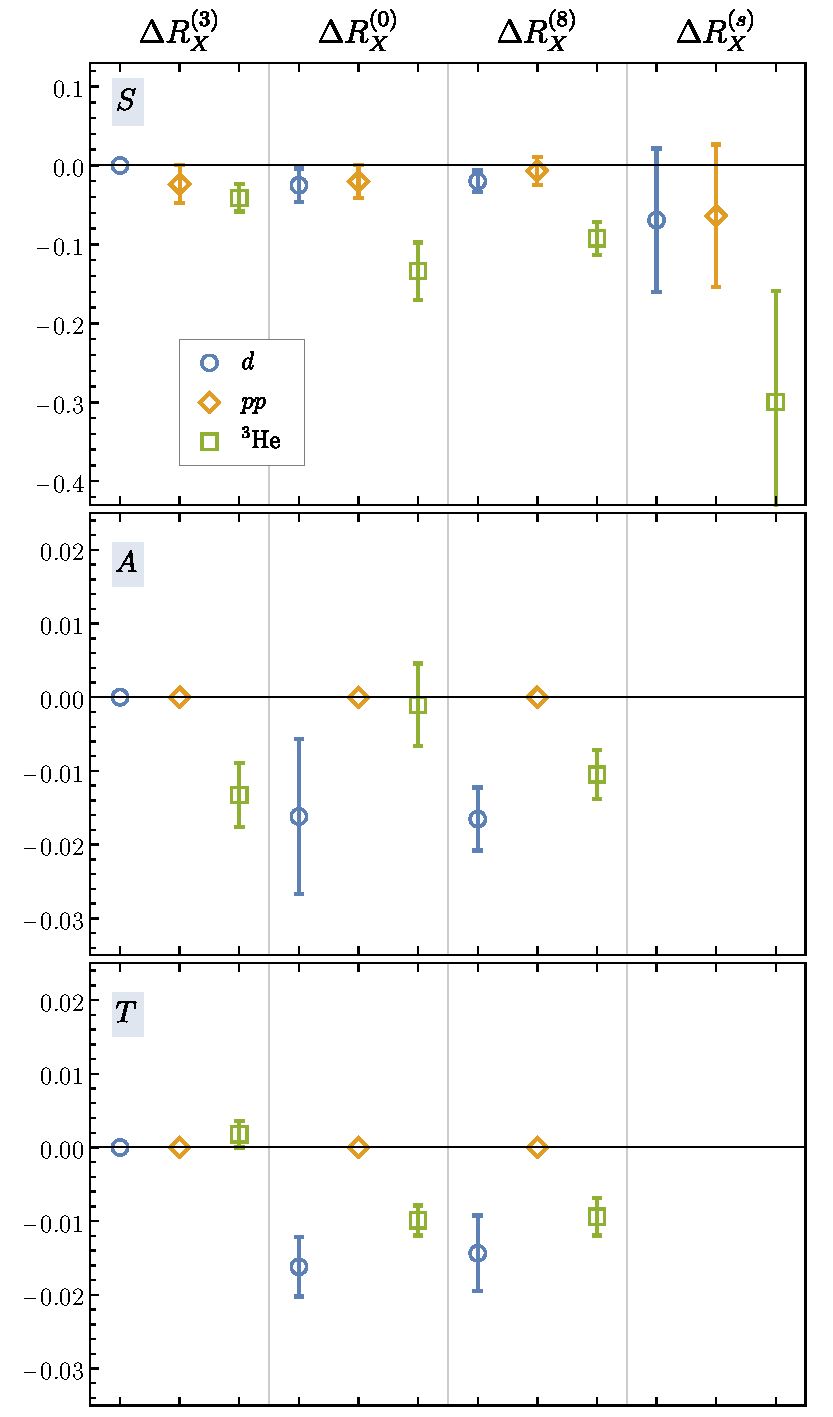
\includegraphics[width=0.4\columnwidth]{figures/RatioSummary.pdf}  
	\caption{ 
		The differences of the scalar, axial and tensor current matrix elements of light nuclei from single particle expectations ~\protect\cite{Beane:2015yha}. Nuclear effects can be identified by the deviation of quantities from zero.   
	}
	\label{fig:SAT}
	\vspace*{-0.5cm}
\end{figure}
%
From the LQCD point of view,  the first steps have been taken in this direction, with isovector magnetic moments \cite{Beane:2014ora,Beane:2015yha,Detmold:2015daa} and magnetic  polarizabilities \cite{Chang:2015qxa} of nuclei up to $A=4$ being computed at heavier than physical quark masses using background field methods. Interestingly, relations that exist between magnetic moments in phenomenology are also apparent in the LQCD resutls at heavy quark masses. For example,  the magnetic moment of the triton is very close to the magnetic moment of the neutron as in the simplest shell-model configuration, the two protons spin pair to zero. The extracted magnetic moments and polarizabilities are summarized in Fig.~\ref{fig:summaryBETA} and as seen in left panel, the close agreement between the LQCD  and experimental magnetic moments is striking.

The Gamov-Teller (GT) contributions to the weak decay of the triton \cite{Savage:2016kon} and the coupling on $A\le3$ nuclei to scalar and tensor currents \cite{Chang:2017eiq} have also been investigated using similar background field techniques. The weak decay of the triton is the simplest nuclear probe of weak interactions and the GT contribution is most uncertain. 
As discussed extensively in the companion White Paper on Fundamental Symmetries, the scalar current is relevant for interactions with nuclei in many models of dark matter~\cite{Undagoitia:2015gya} and for searches for new physics in precision spectroscopy~\cite{Delaunay:2016brc,Delaunay:2017dku}, while the tensor current determines 
the quark electric dipole moment contribution to a nuclear electric dipole moment~\cite{Engel:2013lsa,Yamanaka:2016umw,Chupp:2017rkp} and is thus an important ingredient in searches for new sources of time-reversal violation. 
 The nuclear dependencies of the various currents are shown in Fig.~\ref{fig:SAT}.


While the quark structure of nucleons and nuclei is relatively well probed by electron scattering experiments, unraveling the gluonic structure is vastly more difficult. As idscussed in Section \ref{sec:hadronstructure}, the Electron Ion Collider \cite{Accardi:2012qut}, a major new Nuclear Physics accelerator facility planned for construction in the 2020s, will particularly target the gluon structure of nucleons and nuclei. LQCD calculations can play an important role in planning this facility and setting benchmarks for first measurements of various gluon structure quantities. To this end, a preliminary study of the modification of the lowest moment of the unpolarized  gluon distributions in nuclei, the gluon momentum fraction, has been performed \cite{Winter:2017bfs}, although nuclear effects were bounded rather than resolved.   In addition, the first moment of the gluon transversity structure function was investigated in the spin-1 deuteron. This latter  quantity  corresponds to a target helicity flip by two units and so vanishes for the nucleon; it is therefore intrinsically a nuclear effect.



%FORM FACTORS
Calculations of electroweak interactions with nuclei that include recoil from the currents and thereby determine the input nuclear form factors necessary to constrain  elastic electron-nucleus and  neutrino-nucleus scattering. This will reduce the theoretical uncertainties inherent in the coming long-baseline neutrino experimental program as discussed in detail in the companion White Paper on Neutrino Interactions. Coupled to the calculations of the proton charge radius described above, calculations of the charge radii of the light nuclei $d$, $^3$He and $^4$He  will enable further insight into the discrepancies in nuclear charge radii between muon spectroscopy and electron scattering and spectroscopy \cite{}.


%PARTON
Future calculations will explore the modification of moments of parton distributions in light nuclei, thereby probing the EMC effect from QCD. While these calculations will be in light nuclei, effective field theory \cite{Chen:2004zx,Chen:2016bde} and phenomenology \cite{Hen:2016kwk} suggest that two-body correlations that can be determined in the few nucleon sector are sufficient to describe the EMC effect. LQCD can also help address more complex questions such as the flavor and spin dependence of the EMC effect that are hard to access from phenomenology. Using the techniques described in Section \ref{sec:hadronstructure}, the Bjorken-$x$ dependence of nuclear parton distributions will also be accessible, significantly expanding the connection of LQCD to phenomenology in this area. Further calculations of gluonic properties will reveal exotic aspects of nuclear structure such as double-helicity-flip parton distributions.





\subsection{Nuclear interactions}


Understanding the  forces between nucleons that result in binding into nuclei is a central goal of LQCD studies of nuclei. As discussed in Section \ref{sec:hadronspectroscopy} above, two particle interactions can be addressed using the finite volume formalism of L\"uscher that converts finite volume energy levels into determinations of scattering phase shifts up to inelastic thresholds. Over the last decade, calculations of scattering phase shifts for baryon-baryon systems have become increasingly advanced, although they are still far from the level of sophistication that has been achieved in the meson sector. The two different nucleon-nucleon spin channels ave been studied over a range of quark masses, with the most recent calculations  performed at masses corresponding to $m_\pi\sim XXX$ MeV. Hyperon-nucleon scattering parameters have also been extracted and extrapolated to the physical quark masses.  
Knowledge of the nucleon-hyperon ($n\Lambda$ and $n\Sigma$) scattering phase shifts is  important in determining the equation of state of neutron stars as strongly attractive interactions make it feasible for the dense core of neutron stars to relieve degeneracy pressure through hyperon production. However the unstable nature of hyperons makes it very difficult to extract these phase shifts from experiment. Unlike in $NN$ case, the scattering phase shifts extracted from LQCD rival the precision of phenomenological determinations and indicate that hyperons are potentially relevant in the interior of neutron stars \cite{Beane:2012ey,Wagman:2017tmp}. With recent detection of gravitational wave signatures of a  neutron star merger event and with the first release of observations from the NICER satellite observatory expected soon, QCD input into the nuclear equation of state has taken on a new impetus. In the coming decade such scattering phase shifts will be extracted with full control of systematic uncertainties; calculations of the nucleon-nucleon interaction will benchmark LQCD, while those in more exotic channels will be predictions that challenge experiment and act as input to phenomenology. Future calculations will also include the effects of QED in scattering analyses \cite{Beane:2014qha}.

Say something about Potentials

Three-nucleon forces can also be determined from finite volume spectroscopy.  However the complexity of the three-body interactions means that the amplitude based methods used for two-particle systems are challenging to apply. While the simplest aspects of the formalism needed to extract interactions from three particle finite-volume energies have been developed \cite{Beane:2007qr,Detmold:2008gh,Tan:2007bg,SharpeETC}, as yet the only systems that have been analysed numerically are multi-meson system that interact weakly. At present analysis of three baryon systems must resort to  effective field theory based methods \cite{Detmold:2012wpa,Detmold:2013wda,Detmold:2015jda,Kirscher:2015tka,Davoudi:2017ddj,Savage:2016egr} in which the finite volume eigenspectrum of QCD in the relevant quantum number systems is matched to EFT calculations in the same volume, thereby enabling extraction of the relevant low energy constants. This approach make use of the full statistical power of the LQCD calculations, but relies on the EFT to extract infinite volume physics. Initial EFT studies matching to multi-nucleon ground state binding energies have been undertaken \cite{Barnea:2013uqa,Bansal:2017pwn,Contessi:2017rww,Gandolfi:2017arm}, determining the LECs of the two and three-nucleon interactions in pionless (at a set of unphysical quark masses) and pionful EFTs. Having determined these LECs, the EFTs have been used to extrapolate to larger systems such as $^{16}$O has been possible. Electromagnetic properties have also been used to constrain EFT approaches \cite{Kirscher:2017fqc}.




The electroweak interactions of two nucleon systems are particularly important phenomenologically 
\begin{figure}
	\centering
	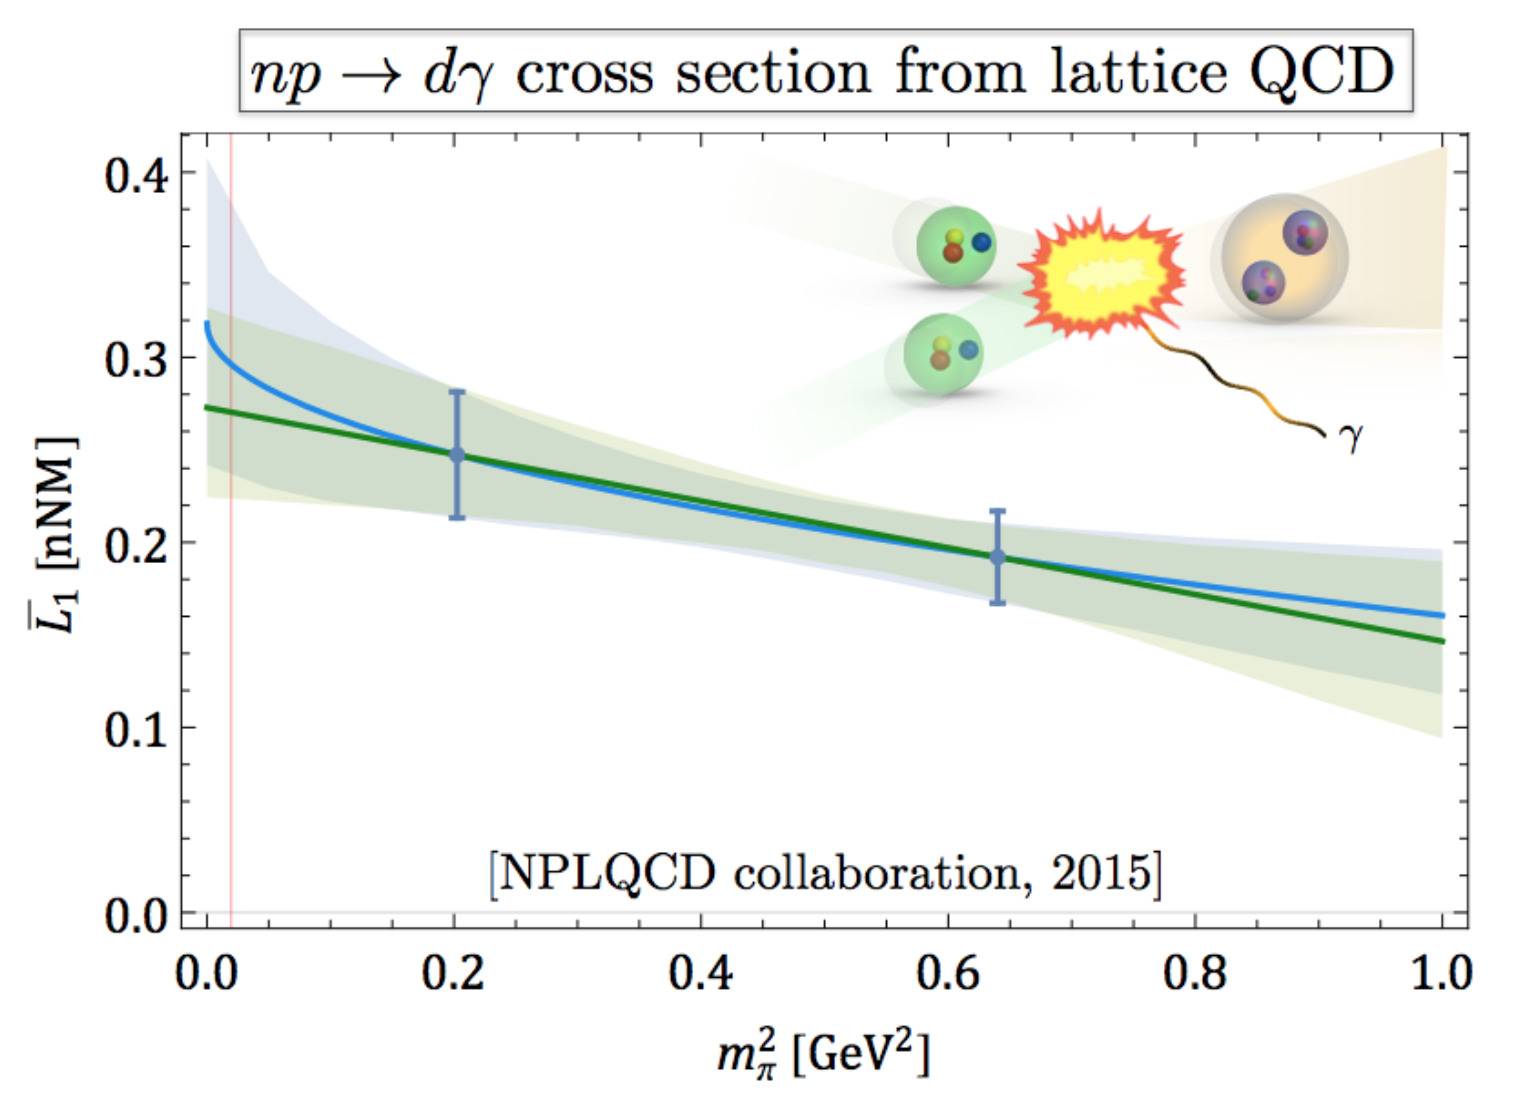
\includegraphics[width=0.48\columnwidth]{figures/npTOdgamma.png}  
	\caption{ 
		The short-distance correlated two-nucleon (meson-exchange current)
		contribution to $np\rightarrow d\gamma$~\protect\cite{Beane:2015yha}.    
	}
	\label{fig:L1bar}
	\vspace*{-0.4cm}
\end{figure}
%
Calculations of two-nucleon systems in external magnetic fields were used to isolate the
short-distance two-body electromagnetic contributions to the low-energy radiative capture process $np\rightarrow d\gamma$,
and the photo-disintegration processes $\gamma^{(*)}d\rightarrow np$~\cite{Beane:2015yha},
as shown in Fig.~\ref{fig:L1bar}. 
In nuclear potential models, such contributions are described by 
phenomenological meson-exchange currents; using LQCD we were able to determine them directly from the quark and gluon interactions of QCD.
This was achieved by calculations of coupled neutron-proton systems in multiple background magnetic fields, at two values of the 
quark masses, corresponding to pion masses of $m_\pi\sim 450$ and 806 MeV. The results were extrapolated to the physical pion mass using pionless EFT, allowing the rate of the low-energy inelastic process to be determined 
at the physical point. 
%Extrapolating to the physical pion mass,
%a cross section of $\sigma^{\rm lqcd} (np\rightarrow d\gamma)=\sigmaPHYS~{\rm mb}$ 
%was obtained 
%at an incident neutron speed of $v=2,200~{\rm m/s}$, consistent with the experimental value of
%$\sigma^{\rm expt}(np\rightarrow d\gamma)=\sigmaEXPT~{\rm mb}$.
%
%
This is the first LQCD calculation of an inelastic nuclear reaction and both it, along with an extension to ~\cite{Beane:2015yha,Detmold:2015daa}. 




ed the first LQCD calculations of the nuclear matrix element determining the $pp\rightarrow d e^+\nu_e$ fusion cross section and the Gamow-Teller matrix element contributing to tritium $\beta$ decay. The method used is very similar to the one that will be needed to achieve the objectives of this proposal.
Using a new implementation of the background field method,
the matrix elements were calculated at the SU(3)-flavor symmetric 
value of the quark masses, corresponding to a pion mass of $m_\pi\sim 806~{\rm MeV}$.Assuming that the short-distance correlated two-nucleon contributions to the matrix element 
(meson-exchange currents) depend only mildly on the quark masses, as seen for the analogous magnetic interactions, 
the calculated $pp\rightarrow d e^+\nu_e$ transition matrix element leads to a fusion cross section at the physical quark 
masses that is consistent with its currently accepted value, although further calculations are required to  better substantiate this conclusion. Moreover, the leading two-nucleon axial counterterm of pionless EFT is determined to 
be $L_{1,A} = 3.9(0.2)(1.0)(0.4)(0.9)~{\rm fm}^3$ at a renormalization scale set by the physical pion mass, 
also in agreement with the accepted phenomenological range. 
This work concretely demonstrates that weak transition amplitudes in few-nucleon systems can be studied directly 
from the fundamental quark and gluon degrees of freedom and  
opens the way for future investigations of many important quantities in nuclear physics. 
\cite{Savage:2016kon} 





For some specific nuclei such as germanium, single $\beta$ decay is energetically forbidden, but double $\beta$ decay is allowed. In the Standard Model, this decay occurs with the release of two electrons and two anti-neutrinos, conserving lepton number  ($2\nu\beta\beta$-decay). In many beyond the standard model scenarios, either with light Majorana neutrinos (particles that are their own antiparticles) or with other forms of lepton number non-conservation at high scales,  a second form of  double $\beta$ decay that involves no neutrinos in the final state ($0\nu\beta\beta$-decay) can occur. Observation of this latter process would be an unambiguous signal for new physics. Understanding of the implications of such an observation, as well as design of future experiments seeking this decay mode, requires understanding the relevant $\Delta I=2$ nuclear transition matrix elements. This is a challenging task and state-of-the-art nuclear theory calculations differ by an order of magnitude. LQCD offers the prospect of providing useful input in this area through calculations of the relevant matrix elements in light nuclei that can be used to control uncertainties in nuclear models. In the last two years, the $2\nu\beta\beta$ process has been studied in the $pp\to nn$ transition \cite{Tiburzi:2017iux,Shanahan:2017bgi},  the pionic matrix elements, $\langle \pi^+ | {\cal O} | \pi^- \rangle$, of $\Delta I =2$ short distance operators \cite{Nicholson:2018mwc}, and the $\pi^-\to \pi^+ e^- e^-$ and $\pi^-\pi^-\to e^-e^-$ transitions induced  by a light Majorane neutrino \cite{Feng:2018pdq,Detmold:2018zan}, have all been investigated for the first time. Future refinements of these calculations, even restricted to few nucleon systems, have the potential to significantly impact experimental search design.  Already  these finding suggests that nuclear models for neutrinoful and neutrinoless $\beta\beta$ decays need to incorporate this previously neglected contribution if they are to provide reliable guidance for next-generation neutrinoless $\beta\beta$-decay searches. 



\subsubsection{Future opportunities}



Scattering  phase shifts of $NN$ systems. validation of LQCD calculations at physical point. Understanding role of Coulomb, eg $a_{pp}$ vs $a_{np}$ vs $a_{nn}$ in the spin singlet channel.

More sophisticated EFT matching 

Light nuclear reactions for the BBN


\subsection{Nuclear input for neutrino physics and fundamental symmetries}


Nuclei are used as targets in intensity frontier experiments that are trying to probe the neutrino sector and to look for physics beyond the SM. In particular, argon ($Z=18$) is the target material for a number of current neutrino experiments and will be the target for the upcoming Deep Underground Neutrino Experiment (DUNE), while a range of nuclei such as sodium ($Z=11$), xenon ($Z=54$) are used in dark matter direct detection experiments \cite{Undagoitia:2015gya}. Charge lepton flavor violation searches look for $\mu\to e$ conversion in the field of aluminium ($Z=13$) \cite{Albrecht:2013wet}, and precision isotope-shift spectroscopy experiments consider a wide range of nuclei ranging from hydrogen ($Z=1$) to ytterbium ($Z=70$) in  order to constrain new physics \cite{Delaunay:2016brc,Delaunay:2017dku}, both requiring knowledge of various nuclear matrix elements \cite{Chang:2017eiq}. Finally, double-$\beta$ decay (DBD) searches utilize heavy isotopes to search for lepton number violation through neutrinoless DBD \cite{DellOro:2016tmg,Engel:2016xgb} as discussed above.

All of the techniques discussed above in the study of nuclear spectroscopy, structure and interactions are applicable in these areas, and calculations are being actively pursued. We leave a full discussion of these topics to the two companion USQCD whitepapers on Neutrino-Nucleus Interactions and on Fundamental Symmetries.



